\documentclass[../practica_02.tex]{subfiles}

\begin{document}

    \begin{enumerate}
        \item $f(x,y) = 3y$

            $ \Leftrightarrow f: \real^2 \rightarrow \real$

            $ un plano $

            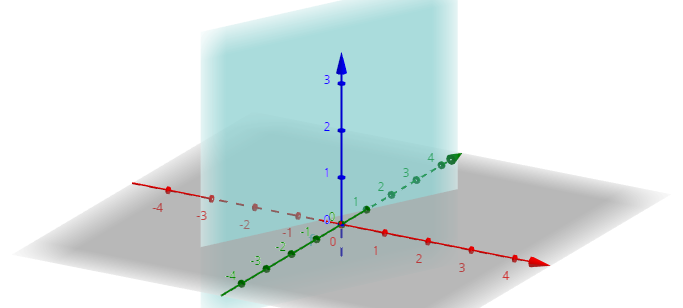
\includegraphics[scale=0.4]{ej13/resources/a.png} $ $
            
        \item $ f(x,y) = \frac{1}{x}$
            
            $ \Leftrightarrow f: \real^2 - (x,y): x = 0 \rightarrow \real$

            $ un hiperboloide $

            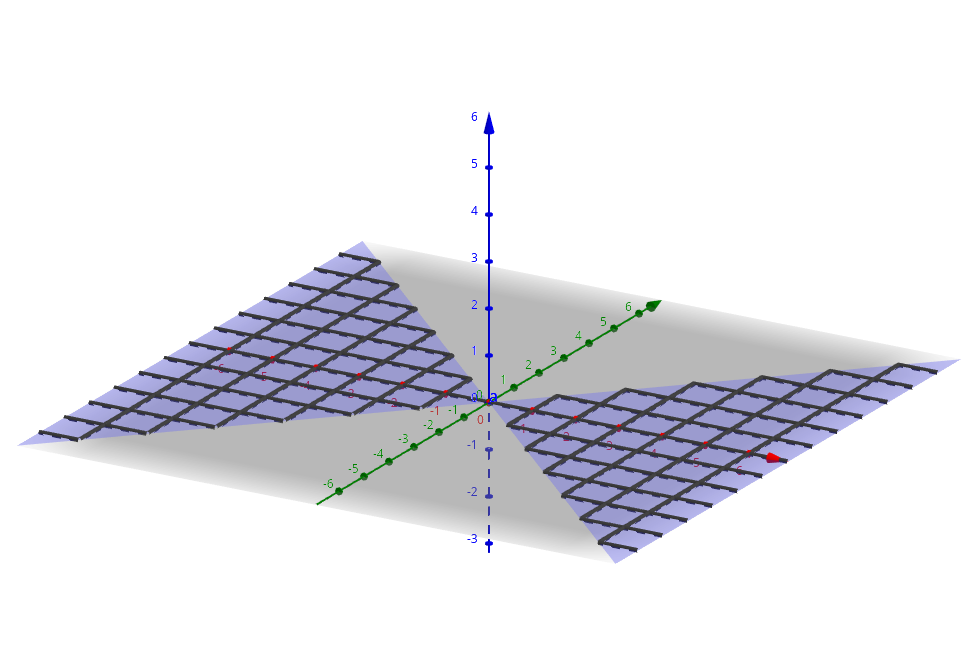
\includegraphics[scale=0.4]{ej13/resources/b.png} $ $

        \item $ f(x,y) = x^2 + y^2$

            $ \Leftrightarrow f: \real^2 \rightarrow \real_{\geq 0}$

            $Un paraboloide$

            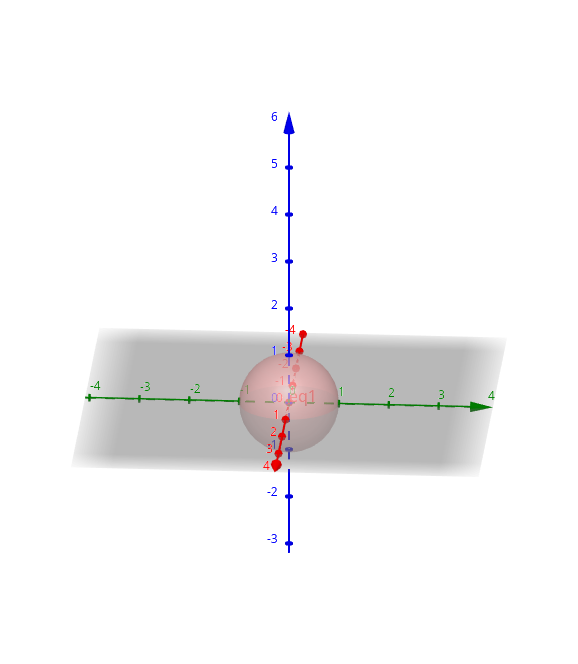
\includegraphics[scale=0.4]{ej13/resources/c.png} $ $

        \item $ f(x,y) = -x^2 - y^2 \equiv - (x^2 + y^2) $

            $ \Leftrightarrow f: \real^2 \rightarrow \real_{\leq 0}$

            $Un paraboloide negativo$

            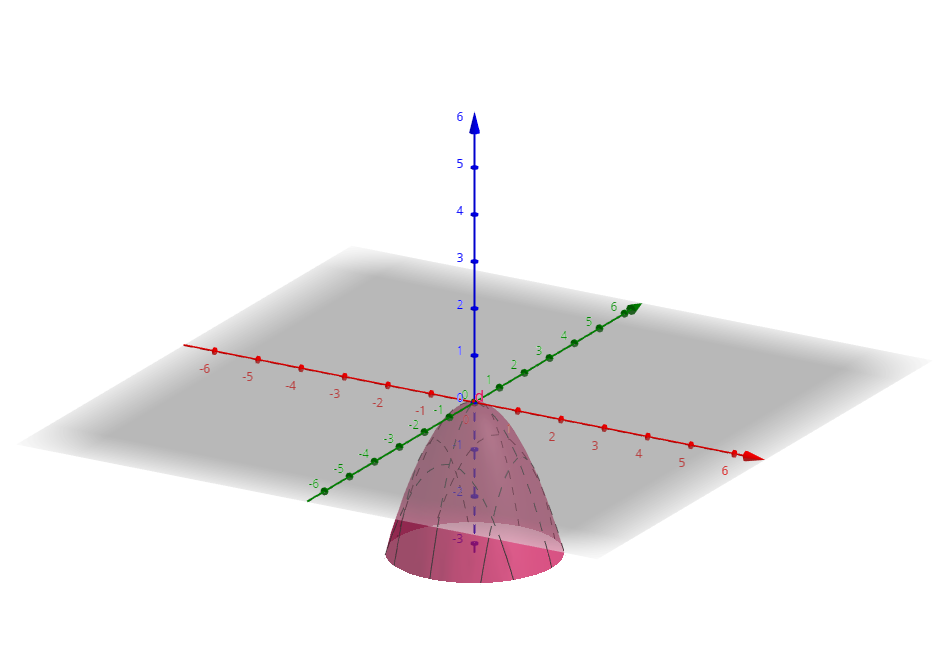
\includegraphics[scale=0.4]{ej13/resources/d.png} $ $

        \item $ f(x,y) = \sqrt{x^2 + y^2}$

            $ \Leftrightarrow f: \real^2 \rightarrow \real$

            $Un cono$

            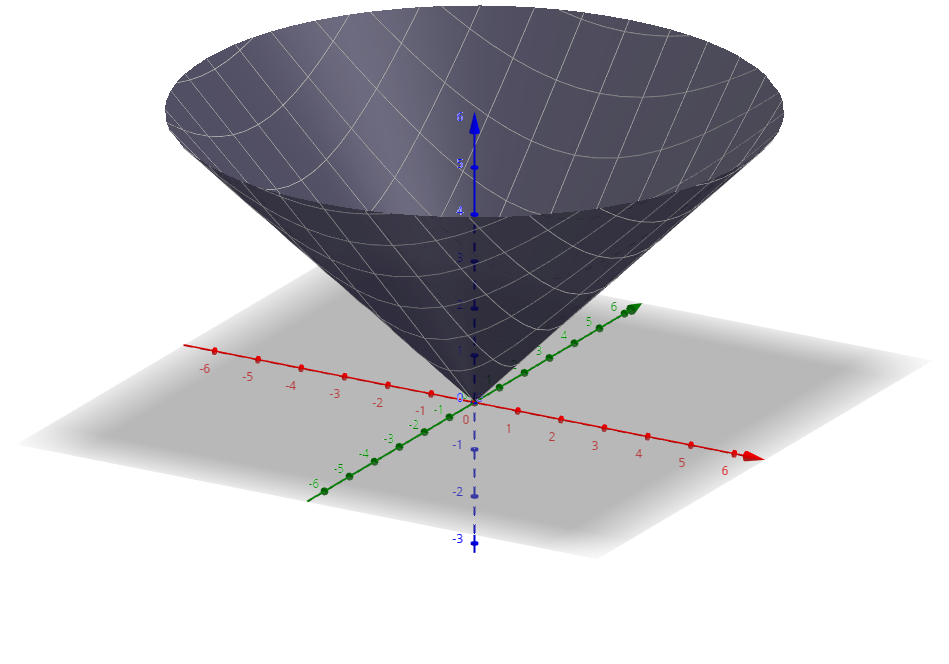
\includegraphics[scale=0.4]{ej13/resources/e.png} $ $

        \item $ f(x,y) = \sqrt{4 - x^2 - y^2}$

            $4 - x^2 - y^2 \geq 0 \Leftrightarrow$
            $ 4 \geq x^2 + y^2 $

            $ \Leftrightarrow f: (x,y) \in \real^2 : 4 \geq x^2 + y^2 \rightarrow \real$

            $Un cono$

            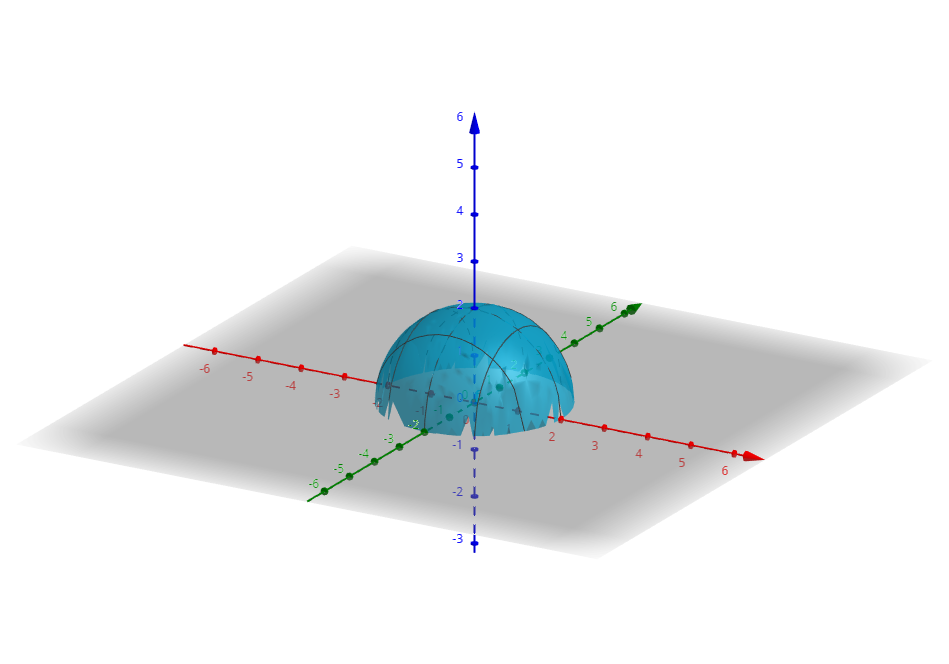
\includegraphics[scale=0.4]{ej13/resources/f.png} $ $

    \end{enumerate}

\end{document}